\documentclass[titlepage]{report}

\usepackage{titlesec}
\usepackage{lipsum}
\usepackage{graphicx}
\usepackage{wrapfig}

%setting for chapter font
\titleformat{\chapter}[display]
  {\Huge\bfseries}{}{1pt}{\Huge}
  
  

\title{\textbf{CustoNN2: Customizing Neural Networks on FPGAs}}  


\begin{document}
\maketitle

\tableofcontents{}
\newpage

\chapter{Introduction}
In recent times Convolutional Neural Networks (CNN) have gained immense popularity and are being used in many applications such as image classification, speech recognition, etc. CNNs have become an industry standard and provide a near-human accuracy. However, CNNs are computationally intensive models requiring a large amount of processing power which calls for the need to have dedicated
hardware for its acceleration. Graphics Processing Units (GPU) are conventionally used and provide satisfactory performance on some of the state-of-the-art CNN models. Although GPU provides good performance, it is not flexible enough to accommodate multiple CNN models. One may need to re-design the entire GPU architecture for a particular CNN. This is where Field Programmable
Gate Arrays (FPGA) proves to be much more beneficial in terms of flexibility
and parallel processing. Some state-of-the-art CNN models such as AlexNet,
VGG16 and ResNet have shown considerable performance gain using FPGAs.
Furthermore, the presence of various Software Development Toolkit (SDK)
in the market such as Intel OpenVINO, Xilinx ML Suite and TVM has helped
the developers to efficiently map their CNN models to the underlying architecture. Due to all of these factors, CNN has become a popular choice for image
classification applications.


\section{Why FPGA}
There are multiple hardware available in the market such as CPU, GPU, ASIC, and FPGA each used for a specific set of applications. Among all of them FPGAs are becoming widely popular and are being used in CNN based applications. Deep Neural Networks (DNN) benefit very much from using FPGA. DNN are math intensive models and FPGAs can be used to execute the mathematical operations involved in DNNs. FPGAs have dedicated DSPs and ALUs to perform such math intensive floating point arithmetic operations. FPGAs are suited for applications which use custom datatypes which is the case in DNN. Also, they provide better latency, parallel processing power, and flexibility among all its counterparts. Using FPGA also has another specific advantage. The advantage is that it can accommodate different CNN models without the need of changing the underlying architecture. CNN models have a streaming architecture that suits well with FPGA architecture.
In this project, we are using the Intel Stratix 10 with 520N scaleable FPGA network accelerator card for our CNN inference on image classification. Paderborn Center for Parallel Computing (PC2) has 32 of this FPGA and our task is to scale our CNN architecture using all 32 FPGAs. We will be using three pre-trained models namely GoogleNet, ResNet-50 and Inception-v4 in a model ensemble architecture where majority voting is used. The workload will be divided among all the 32 FPGAs and the layers will be distributed to each of these FPGAs in a streaming architecture fashion. At last, we will measure the performance of our system using some performance metrics.

% Remove below lipsum command before posting your work

\chapter{Goals}
Convolution Neural Network (CNN) is a type of Deep Neural Network (DNN) used in the field of image processing and image analyzing. CNNs are most widely used for extracting valuable features from the input images. The primary goal of our project is to implement the state of the art CNNs on the FPGAs which acts as an accelerator for compute-heavy neural networks. We have the following sub-goals:
\section{Scaling over multiple FPGAs}
An FPGA is made up of finite and limited resources and implementing these large CNN models can often result in running out of resources and cannot fit into a single FPGA. Hence in this project, we will use the FPGA infrastructure in the Noctua cluster. The Noctua cluster is a high-performance computing system equipped with 32 Intel Stratix 10 FPGAs with point to point connections. We will be scaling our CNN models on the Noctua cluster by partitioning the large model into smaller models based on the number of layers that will fit onto a single FPGA and these smaller models can then be executed on multiple FPGAs to provide low latency computation. We will use the OpenCL external IO channels to transfer intermediate results from one FPGA to another. Since we are developing an ensemble of three CNN models, all three can be executed in parallel on different FPGAs and results can be aggregated at the end. By scaling our application on multiple FPGAs infrastructure we target to perform as good as the Microsoft's Project Brainwave architecture in terms of latency and throughput.
\par
Microsoft Project Brainwave is a deep learning platform for real-time Artificial Intelligence (AI) applications like computer vision. Brainwave is equipped with Intel Stratix 10 FPGAs in the Microsoft Azure Cloud and Neural Processing Units (NPU) architecture for executing a DNN model with low latency and high throughput. Brainwave also supports multiple FPGAs infrastructure in the Azure cloud. When the memory resource of the FPGA is exhausted by the DNN model layers, the remaining layers will be mapped to the next FPGA enabling scaling.

\section{Performance Optimization}
Heterogeneous computing systems provide performance gain by using specialized capabilities of different types of processors (CPU+FPGA in our project). OpenCL is a framework for heterogeneous computing which provides software-centric development flow for FPGAs and obtains performance and power advantages with hardware acceleration. We will use the OpenCL tool flow for developing CNN models in our project. It offers us to develop individual kernels for each layer of the CNN model and we will also make use of the channels concept offered by OpenCL to transfer intermediate results from one layer to the next layer without writing the results in the global memory. The kernels will be further optimized by using several OpenCL optimization techniques learnt during the tutorial phase eg: loop unrolling, reducing the Initiation Interval (II) of loops to 1, removing memory dependencies, etc. Performance modeling is applied to each OpenCL kernels to identify the bottlenecks in the design and resolve the issues to obtain a high throughput and high utilization.

\section{Quantization }
CNN implementation is often complex due to the number of parameters and computations, which makes it difficult to be implemented on a resource-constrained FPGA. The floating point operations are computationally too expensive, hence quantization can be applied to the deep networks to convert the floating point weights into fixed point weights. Fixed point operations typically consumes fewer hardware resources than floating point operations. Quantization will help in reducing the power consumption, memory footprint and resources utilization. In our project, we rely on the machine learning suite to optimize and quantize the CNN model so that the accuracy is not drastically dropped in the quantized model. We will also distinguish the models with quantized weights and floating point weights.

%End of the chapter

\chapter{Metrics}
Our objective is to leverage the infrastructure available at the Paderborn Centre for Parallel Computing (PC2) to build an inference accelerator system. We plan to evaluate the effectiveness of our inference accelerator system by considering two classes of metrics - performance metrics and quality metrics.  

Performance metrics just account for the arithmetic operations performed on the FPGA. They do not tell whether the operations being performed are functionally correct or not. To account for the quality of the operations being performed, we also have to consider accuracy, which is defined a little further down in this chapter. Since we will be using existing, pre-trained network topologies, our aim would be to attain (or reach as close as possible to)  the accuracies mentioned in the literature.

\section{Performance Metrics}

\subsection{Operations per cycle}
Operations per cycle is a unit of measure for the numerical computing performance of a computer. Typically expressed as OPs/cycle, this metric tells us how many operations are performed in one cycle.  

To calculate OPs/cycle we look at the source code and the final profiler report from the executed code. From the source code, we calculate the number of operations sans the overheads (loop index calculations, loop increment operations, etc). And from the profiler report, we get a concrete idea of the clock frequency of the FPGA and the execution time. Combining these two allows us to calculate operations per cycle.

\subsection{Operations per second}
Operations per second is closely related with the above metric “Operations per cycle”. It is usually expressed as OPs/second. OPs/second depends on the clock frequency of the platform. 
We calculate “operations per second” by simply dividing the number of operations by the execution time.  
As per literature mentioned in chapter 7 Related Work, popular tool-flows like DNNWEAVER on Arria 10 GX115 have achieved 184.33GOPs/second, running at a clock frequency of 200MHz.

\subsection{Operations per byte}
Operations per byte or Arithmetic Intensity is the number of operations performed per a byte of data transferred between the FPGA and off-chip memory.  
In our case, we calculate the number of operations performed and the total amount of data transferred by looking at the source code. We also look at the profiler report at the end of execution to get the correct estimation of data transferred between global memory and local memory.  
This metric helps us identify if we are memory bandwidth limited or compute resource-bounded.  

The metrics OPs/second and OPs/byte make up the metrics required to do Roofline Analysis of our inference system.  


\subsection{Latency}
Latency is generally defined as the time delay between initial input to a system and the output from the system. Latency captures the time it takes to load data, pre-process it, send said data over a network to the Inference Engine, the time needed for inference, and time needed to send the classified data back to the user.   

Latencies can be measured for just a single image or over for a batch of images. We can expect to have different latencies based on how we measure it (single image vs batch of images).  

As an example of what has been achieved in related works, we have ALAMO tool-flow running on Arria 10 GT115 running at 239.62MHz having a latency of 4.05ms.
Our aim would be to have latencies in this range.

\subsection{Throughput}
Throughput is a measure of the amount of information processed per unit time. In our case, we define it as the number of images classified per second.  There are well-known techniques to improve throughput like batch processing where a number of images are batched together and sent for inference job. 
But as the batch size goes up, latencies also tend to go up. So there is a trade-off involved here between throughput and latency.  \par
We had deployed a pre-trained ResNet50 DNN model in the Microsoft Azure cloud during our research phase and the images were classified in less than 4 ms and throughput of 39.5 Teraflops on a single Stratix 10 FPGA. Hence we decided to benchmark our project group's implementation against Project Brainwave.



\section{Quality Metrics}
\subsection{Accuracy}
Accuracy is defined as the fraction of the number of correct inferences made to the total number of inferences made. In our context, accuracy depends on the CNN topology used, nature of weights (floating point vs fixed points, etc), training data, etc. 
In literature, accuracies are expressed in terms of percentages and the changes from baseline models' accuracies are measured in terms of percentage points (pp). 
The use of quantized weights in our project might decrease the accuracy compared to baseline models. In our case, baseline models are the existing, trained topologies mentioned in chapter 3. Our goal would be to make use of DNN approximation techniques and still achieve accuracy within 3pp of the baseline model.


\subsection{Rate Correct Score}
Taking inspiration from the field of Memory and  Cognitive research, we can combine accuracy and latency by considering Rate Correct Score. It is defined as    

$RCS = \frac{c}{\sum R_t}$    

where   

$c$ = accuracy    

      $\sum R_t$ = batch execution time  
      
Our aim would be to maximize RCS (either by increasing the accuracy or by decreasing the latency or both).

%End of the chapter

\chapter{Datasets, Topologies and Architecture comparison}

\section{Datasets}
CNNs are trained on datasets. Each dataset consists of specific type of images and each of them is used in different tasks such as image classification or image captioning etc. Below are some of the datasets specified which we can choose to work on in this project.
\subsection{ImageNet}
It is one of the most prominent datasets used in the field of visual object recognition. In 2009 this dataset was first introduced to the world in the Conference on Computer Vision and Pattern Recognition by the computer science department of  Princeton University. It has over 14 million images and over 20000 categories. A large portion of the images has been hand annotated which can be helpful in the task of image captioning. Every year ImageNet runs a challenge called the ImageNet Large Scale Visual Recognition Challenge (ILSVRC), where different software architectures and algorithms take part in order to classify images of the dataset correctly. By 2017 most of the algorithms working on ImageNet have already achieved the accuracy of more than 95\%.

\subsection{CIFAR10}
CIFAR named after Canadian Institute For Advanced Research is a widely used dataset in machine learning paradigm which is used in training various machine learning models. It is used in visual object recognition. It consists of 60000 images in total. The 10 in the name stands for the 10 classes in the dataset and each class has 6000 images. Each image in the dataset is of 32*32 pixels coloured images. The 10 classes in the data set are air-planes, cars, birds, cats, deer, dogs, frogs, horses, ships, and trucks. Since the images in the dataset are of low resolution, it is one of the favourites for researchers to train their algorithms since they do not have to invest huge amount of resources in terms of money and hardware infrastructure. 

\subsection{MNIST}
Modified National Institute of Standards and Technology is a dataset consisting of handwritten digits. This database is commonly used in the field of machine learning. MNIST is a derived dataset from NSIT dataset. It consists of images which are 28*28 pixel size and greyscale nature. This dataset has been divided into 2 sets. To say in total it has 60000 training images and 10000 testing images. NSIT's testing dataset contributes to one half of the training and testing database of the MNIST and the other half is filled by NSIT's training dataset. The lowest possible error rate on MNIST achieved is 0.23\%
which was done by implementing a system of CNNs.

\subsection{Selection of Dataset}
Reasons for selecting ImageNet are as follows:
\begin{itemize}
    \item The topologies that are going to be used in the project are well optimized for ImageNet. Hence CIFAR10 and MNIST are not being considered also also they don't pose a significant challenge in testing and training complex CNNs.
    \item On the other hand, ImageNet provides a greater challenge and also the topologies that are going to be used have already used ImageNet dataset. Hence their result can be used as a benchmarking performance for the implementation in the project.
\end{itemize}

%End of the chapter


\section{Topologies}
Here, we describe the CNN topologies that we will be deploying in our project. These are some of the state-of-the-art topologies that have performed exceptionally well on the ImageNet challenge such as ResNet and GoogLeNet, as a result of which we made the decision for their deployment so as to investigate how their performance can be improved through FPGA acceleration while maintaining classification accuracy. The following sections give a detailed explanation about their architectures and basic working principles.
\subsection{GoogLeNet}
GoogLeNet is a deep convolutional neural network and is also known as Inception-v1. The architecture is based on the Hebbian principle which states that \textit{cells that fire together wire together} with the intuition of multi-scale processing. GoogLeNet is 22 layers deep network and used for object detection and classification. It has modules known as Inception which is a network within a network. GoogLeNet does not have any fully connected layers but uses global average pooling which keeps the model from overfitting the data. It was able to achieve a top-5 error rate of 6.67\% and requires only 4 million parameters, whereas AlexNet requires up to 60 million parameters.

\subsubsection{Inception Module}
The logic behind Inception architecture is built on finding optimal local sparse structure in the convolution network and to repeat it spatially. There are 9 inception modules in GoogLeNet. Each inception module has 6 convolution layers and 1 max pooling layer. Some convolution layers and max pool layer are stacked on each other due to which four different outputs are created within the inception module which is concatenated to produce one single output and it is passed to next inception module and so forth. Concatenation of this output filter occurs based on depth wise. The 1x1 convolution layers in inception module help us to preserve spatial dimensions and to reduce the feature depth.

The output from the last inception module is forwarded to global average pooling.

\begin{figure}[h!]
    \centering
    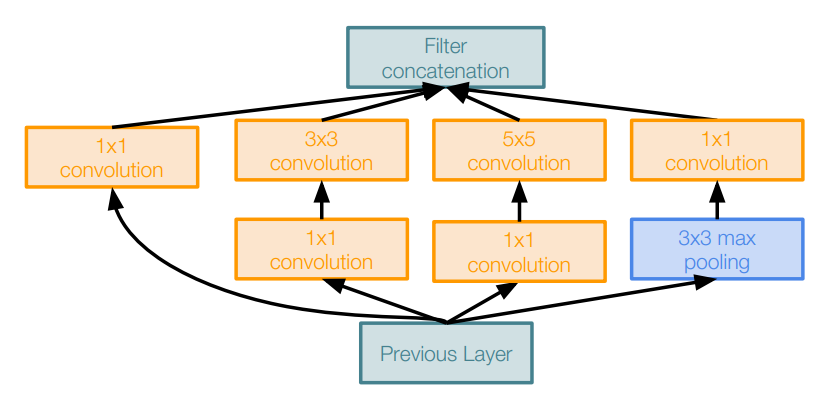
\includegraphics[scale=0.4]{googlenet}
    \caption{Inception Module}
\end{figure}

\subsection{ResNet 50}
ResNet is a deep neural network released by Microsoft and, also a winner of the ILSVRG 2015 in image classification, detection, and localization. ResNet is a series of DNN with different number of layers from 18 to 152. The base idea is applying the residual connections which are described as learning the residual representation of functions instead of signal representation. One of the conceptual ideas of ResNet is using the skip connection. Skip connection makes the network deeper.  
\begin{figure}[h!]
    \centering
    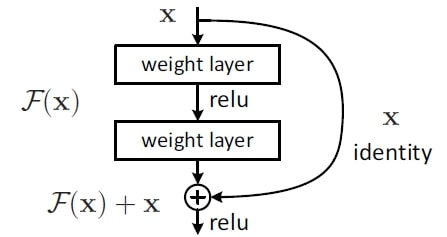
\includegraphics[scale=0.4]{resnet_1}
    \caption{Skip connection}
\end{figure}

Many convolution DNNs run into a problem with vanishing or exploding gradients because, during backpropagation, we derive error function with respect to the current weight and get multiplying of small or large numbers. The product of small numbers will be zero (vanished) and the product of large numbers will be too large (exploded). Developers of ResNet solved this problem by using a skip connection. In the skip connections for the next layer, they use the input from the previous layer without any modification. 


\begin{wrapfigure}{l}{0.4\textwidth}
\centering
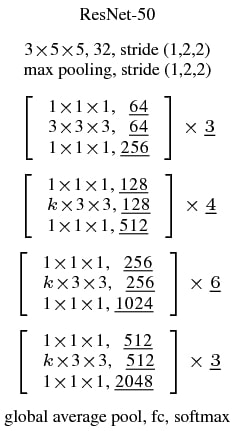
\includegraphics[scale=0.5]{resnet_2}
\caption{ResNet-50}
\label{fig:resnet_50}
\end{wrapfigure}

The output of skip connection is  F(x) + x and the weight layers actually are to learn a kind of residual mapping: output minus identity x. If we have a vanishing gradient we always have an identity x to send it back to previous layers. 

After each convolution layer, ResNet uses the batch normalization from Inception-v2. 

The main concepts of constructing ResNet:
\begin{itemize}
\item Avoiding representational bottlenecks by not abruptly reducing the dimension of data, but smoothly from the beginning of the network to the classifier at the output.
\item Factorization of convolution layer into smaller pieces because this will save resources and help to increase the count of layers.
\item Supporting a balance between the depth and width of the network. You should increase or decrease both dimensions.
\end{itemize}

Figure \ref{fig:resnet_50} shows the whole scheme for ResNet-50.

\subsection{Inception-v4}
Inception-v4 is a deep neural network (DNN) released by Google. Inception-v4 is the fourth version of inception module and includes all techniques from Inception-v1, Inception-v2, and Inception-v3. Google devised inception module and it was a key idea for Inception-v1. The naive version of the first inception module included 1X1, 3X3 and 5X5 convolution and max-pooling as input and the result of them concatenated together as output. \\

The contribution from Inception-v2 is batch normalization. They use ReLU as activation function in order to avoid the saturation problem and vanishing gradients. They had to use a higher learning rate for regularization because the output became more irregular. Last changes were reducing dimension by replacing  5X5 convolution to two 3X3 convolutions. 

Inception-v4 also used the factorization from the Inception-V3. They reduced the dimensionality and it helped to decrease the overfitting problem. For example, if you have a 3×3 filter then you need 9 parameters, but the factorization idea proposes to operate  3X1 and  1X3 filters and use only 6 parameters. 

Inception-v4 has 3.1\% in Top-5 error rate and this result is better than the winner of the 2015 year ResNet (3.57\%) and  Inception-v3 (3.58\%). 

Inception architecture has a relatively low computation cost. Google tries to make the inception module more efficient, so they made it deeper and wider than Inception-v3 and they also simplified the architecture of this DNN.

Figure \ref{fig:inception_v4} shows the whole scheme for Inception-v4.

\begin{figure}[h!]
    \centering
    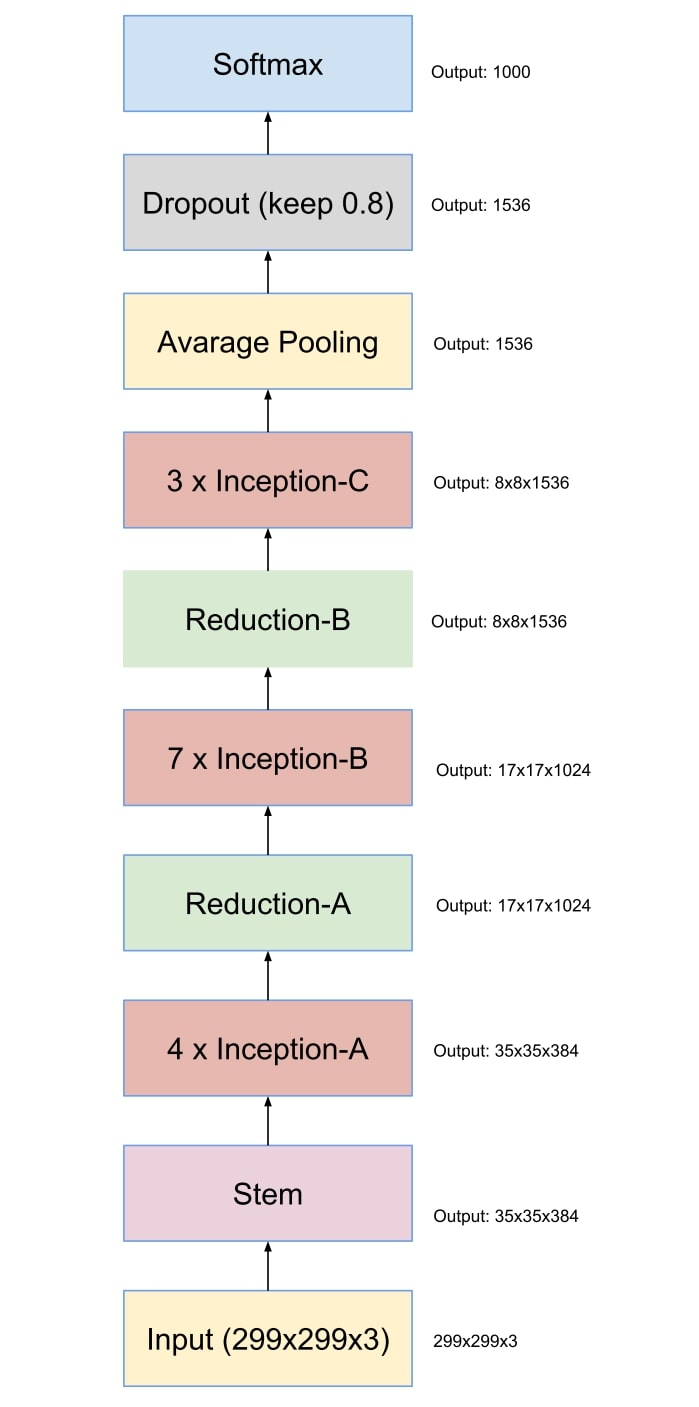
\includegraphics[scale=0.3]{inception_v4}
    \caption{Inception-v4}
    \label{fig:inception_v4}
\end{figure}

\section{Ensemble plan}

We use topologies described above for image recognition and the results obtained with each topology contain several labels and their scores. We choose a label based on its score. In our case, we have three different topologies from which we get three labels and select the one which was found more than one time or have the highest score among all labels. 

Figure \ref{fig:topology_results} shows the example of the output for one of the topologies for the image recognition.

\pagebreak
\raisebox
\begin{figure}
    \centering
    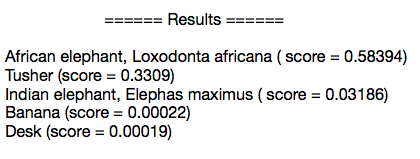
\includegraphics[scale=0.8]{topology_results.png}
    \caption{List of labels with their scores}
    \label{fig:topology_results}
\end{figure}


\pagebreak


\chapter{Technologies}
We have considered the state-of-the-art toolkits to deploy pre-trained deep learning models to execute them on FPGAs as well as to generate OpenCL code.

\section{OpenVINO}
\begin{figure}[!]
    \centering
    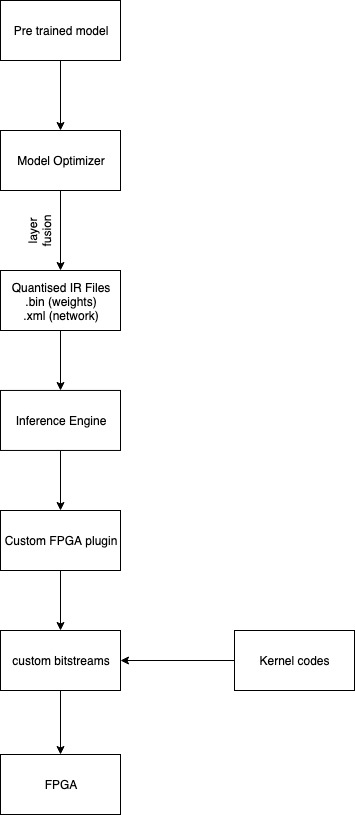
\includegraphics[scale=0.65]{open_vino_flowchart.jpg}
    \caption{OpenVINO Flowchart}
\end{figure}

% Remove below lipsum command before posting your work
Intel OPENVINO is an open source toolkit from Intel that allows the deployment of pre-trained deep neural networks on different hardware platforms such as CPU, GPU, FPGA, etc. The toolkit is available for installation for the Windows operating system as well as selected Linux distributions. All of the tool's libraries and plugins except the FPGA plugin are a part of the open source GitHub repository.
The functionality of OPENVINO is divided among its components, Model Optimizer, Calibration Tool,  Inference Engine. This is shown in Fig 5.1 and explained below. 

\subsection{Model Optimizer}
The Model Optimizer is a python based tool which takes as input a pre-trained model. It supports many popular deep learning frameworks such as TensorFlow, Caffe, PyTorch, MXnet, etc. This model is then converted to a common intermediate format (IR), thereby making the inference engine independent of the training framework. The IR contains a .xml file which represents the computational graph of the CNN and a .bin file containing the weights. The graph is optimized by fusing different layers of the original topology wherever possible. The weights are accordingly adjusted. The toolkit comes with a model downloader which can download various openly available pre-trained models for different frameworks.
 
\subsection{Calibration Tool}
The Calibration Tool, added in the recent release of the toolkit, performs post training quantization to int8 before the IR is passed on to the inference engine.  The tool is open source. 
 
 \subsection{Inference Engine}
 The Inference Engine is responsible for the execution of the model on the selected hardware. For this purpose, it provides a C++ API which can be integrated into an application. The main task performed by the inference engine is to read the intermediate representation of the model, select the hardware for deployments such as CPU or FPGA and call the appropriate plugin which defines all necessary data structures and functions required to perform inference and return the output along with performance statistics. 
 The toolkit comes with pre-compiled bitstreams (.aocx files) for a few supported FPGA boards. These bitstreams implement various popular network topologies such as GoogLeNet, ResNet, etc. as well as generic layers which are used to program the FPGAs as per the requirement of the given model topology.
 
 \subsection{Advantages}
  
 \begin{itemize}
 \item Supports optimization of models and quantization of weights.
 \item A CNN model can be deployed on hardware with minimal programming effort and independent of the training framework.
 \item For FPGAs, the use of pre-compiled bitstreams eliminate the time needed for synthesis of kernel codes.
 \end{itemize}
 
 \subsection{Disadvantages}
 \begin{itemize}
 \item The main disadvantage is the compatibility of FPGA boards. Development and synthesis of kernel codes along with a plugin for FPGAs may be required to make OPENVINO work with unsupported boards. 
 \item Scaling to multiple FPGAs, which is one of the goals of this project is non-trivial as it would require the development of overlays for external I/O channels. 
 \end{itemize}
\section{TVM}

Today we have a lot of different deep learning frameworks such as TensorFlow, Caffe2, MXNet and PyTorch and hardware targets: CPUs, GPUs, FPGAs, and ASICs. During the mapping of one of the frameworks to a device, we run into the problem with a variety of hardware characteristics such as memory organization (implicitly managed, mixed, explicitly managed) and compute primitives (scalar, vector, tensor).

TVM takes the model from different learning frameworks and generates optimized code for devices. TVM was started as a research project at the Paul G. Allen School of Computer Science and Engineering, University of Washington.

TVM includes a computational graph rewriter, tensor expression language and new features for GPU accelerators. The TVM compilation stack is shown in Fig 5.2.

The system has the stack of implementation: NNVM $\to$ TOPI $\to$ TVM $\to$ VTA. NNVM acts as a graph optimizer by taking the model from an existing framework and converting it into “TVM” graph. For these operations, we use the TOPI language. TOPI is a library where functions operate as instructions for further work. For example, TOPI defines a tensor computation, schedules space for each NN operator (e.g. conv2d). The next step is the application of the TVM functions. TVM uses the TOPI instructions and generates code for several backends, such as LLVM, or CUDA, etc. The final step is the Versatile Tensor Accelerator (VTA) which is responsible for the stream and microkernels. 

In order to change a hardware target ( CPU, GPU or TPU) we need to rebuild TVM libraries again.  

\begin{figure}[h!]
    \centering
    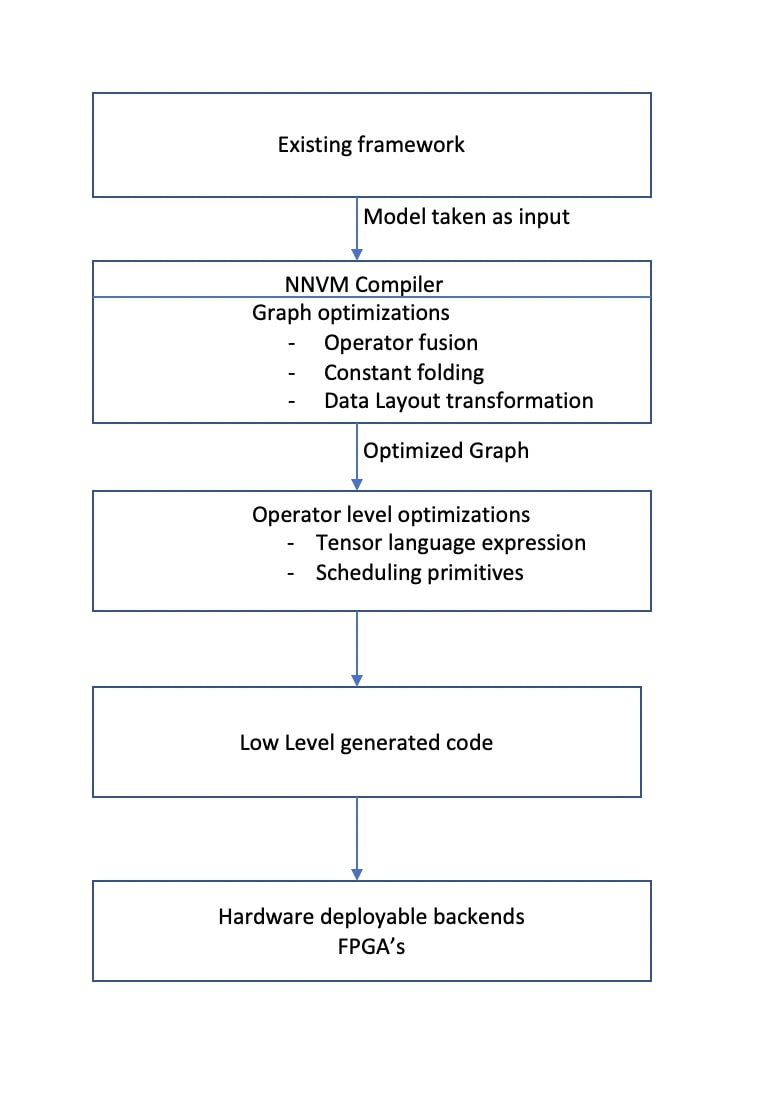
\includegraphics[scale=0.30]{TVM.png}
    \caption{TVM Flowchart}
\end{figure}
 
 \subsection{Advantages}
 \begin{itemize}
 \item TVM is an open-source product.
 \item TVM supports AOCL backend, but this option is still experimental. Information was updated in October 2018.
  \item It is planned to implement a different quantization schemes (Symmetric, Asymmetric, Channel-wise Scale) for different bits (i8 $\to$ i32, i16 $\to$ i32, i8 $\to$ i24, i5 $\to$ i16).
 \end{itemize}

 \subsection{Disadvantages}
 \begin{itemize}
 \item There is no information about which FPGA boards are supported by TVM.
 \end{itemize}

\section{Xilinx}
Xilinx Machine Learning Suite toolchain provides us tools to develop and deploy machine learning applications in real-time inference. It provides machine learning inference with low-latency and high throughput. The suite also provides support for widely used machine learning frameworks such as Caffe, Tensorflow, MXNet.

The functionality of ML-Suite is divided among its components: Machine Learning Framework, xfDNN Middleware, and xDNN IP.

\subsection{Machine Learning Framework}
Xilinx ML Suite supports various frameworks such as Caffe, Tensorflow, Keras, MXNet, Darknet. Support for various other frameworks can also be provided with the help of \textit{Open Neural Network Exchange} (ONNX).

\subsection{xfDNN Middleware}
It is a high-performance software library and provides API which works as a bridge between xDNN IP which runs on FPGAs and ML frameworks such as Caffe, Tensorflow. xfDNN requires SDAccel reconfigurable acceleration environment for running it on Xilinx FPGAs and currently is the only middleware available for programming ML frameworks on Xilinx FPGAs. xfDNN middleware has the following components:
\subsubsection{Compiler}

It provides tools for network optimization such as layer fusions, memory dependency optimization, removing CPU host control bottlenecks with network pre-scheduling. It creates a one-shot execution flow for the network to run on FPGA.

\subsubsection{xfDNN Quantizer} 

xfDNN Quantizer enables fast, high-precision calibration to lower precision deployments to INT8 and INT16. It performs a quantization technique known as re-calibration.

\subsection{xDNN IP}
Xilinx xDNN IP cores are high-performance general CNN processing engines. Various different types of CNN networks and models can be executed on these engines. They have two DSP Array configurations available (28x32 and 56x32). 28x32 configuration provides higher throughput whereas 56x32 can fit larger models at low latency.
xDNN provides \textit{Overlay} to combine various xDNN IP kernels.

\subsection{Advantages}
  
 \begin{itemize}
 \item Supports model optimization and weights quantization.
 \item Delivers high throughput and low latency.
 \item Compiler and Quantizer can run as a single module independent of the environment.

 \end{itemize}
 
\subsection{Disadvantages}
 \begin{itemize}
 \item Does not support fully connected and softmax layers.
 
 \end{itemize}

%End of the chapter

\chapter{Related Work}
% Remove below lipsum command before posting your work
A lot of research has been going on in the field of enhancing the computation speed of CNNs on FPGA for quite some time. In this section, we will take a look at the various research work that has been done so far. We know that CNNs consist of different layers such as convolution, pooling, and fully connected layers, out of which convolution forms a major part of it. C. Zhang et.al implemented convolution layer using sequential nested \textit{for} loops. In our project, we are also using sequential nested for loops for the implementation of convolution layer.

We also know that FPGAs and ASICs increase the speed of inference, while GPUs still excel at floating point operations. CNNs generally work on floating-point representation but working with them comes at a cost in the form of computation time. The need of the hour is to have high throughput and high efficiency. Hence it is better to use data in a fixed-point representation. To cite a few, most of the research work of Jacob et al., Courbariaux et al., Qiu et al., and Shin et al. (2015) has been done in the field of quantization in order to improve computation speed through low bit representation. Courbariaux et al. (2015) implemented block floating point and their CNN topology gave a 1.0 pp accuracy loss. Qiu et al. (2016) used an 8-bit representation of weights on ImageNet and achieved a 0.4 pp accuracy loss. Similarly, other techniques like binarization, ternarization, etc, are also implemented and these techniques showed better performance than the standard CNN which used FP32 bit representation. In our project, we are going to quantize weights in 16-bit representation because by doing quantization of weights in 16-bit we will have a mere loss of 0.1pp in accuracy and also it will help us to achieve our goal of high throughput.

In 2018 a survey was carried out which discussed various tool-flows for mapping of CNN on FPGAs. These tool-flows were distinguished into two categories based on the architecture each tool-flow adheres to. First architecture is \textit{Streaming Architecture} where each layer is assigned a hardware block and these layers are chained to form a pipeline. Second architecture is \textit{Single Computation Engine} architecture which is used to form an overlay. Due to this, it provides flexibility, portability, fast configuration time. In our project, we are aiming to create overlays, where we will create a separate .aocx file for each layer and then these can be called in the OpenVINO plugin to deploy it on FPGAs.


%End of the chapter

\chapter{Time plan}
In this section, we describe how we intend to plan and monitor our project. Since the tutorial phase and research phase were well managed and organized by our mentor Tobias, the scope of this section is limited to the second phase of the project. This section is divided into several parts and each part explains the project’s organizational decisions. 

\section{Project Meetings}
% Remove below lipsum command before posting your work
Project meetings will be held twice a week. Currently, it is being held on Mondays (1 pm to 4 pm) and Wednesdays (9 am to 12 pm). In these meetings, all the project members gather and discuss the current updates in the project. It mainly covers three things. Firstly, the general project updates. Secondly individual task updates where each participant updates about his/her work to the team. Lastly, the issues being faced. 
After each meeting, the minutes of the meeting will be prepared by one of the team members. The assignment of this task is based on round robin fashion. All MoMs will be uploaded to the project’s Git repository.


\section{Project Phases}
\subsection{Project Planning}
% Remove below lipsum command before posting your work
In this phase, we decide on the goals, feasibilities of achieving these goals, prioritizing and the overall organization of the project which will be followed till the completion of the project. This involves defining the scope, dividing the project into subgroups, assigning roles and responsibilities (such as project lead, Git master). Here we define the phases and also estimate the time required. 

During the research phase of the project, the team members conducted background research on 4 frameworks. They were Intel OpenVINO, Xilinx ML Suite, TVM and Microsoft Project Brainwave. While making the project plan, we discuss the feasibilities of each of these tools, pros, and cons from the knowledge gained from the research phase. We identified a design that is a combination of TVM and OpenVINO to achieve our goals. Based on this design, we have come up with three milestones for the project. The details of this and the milestones will be discussed in the next sections. 

The team is working in groups now with one group working on OpenVINO plugin development while the other group is working on using TVM to generate OpenCL kernel for a simple CNN topology. Once this is done, we will identify individual tasks and the team leader will assign them to the members. The track of individual tasks will be kept in MoMs and GitLab. We are using the Waterfall model since it is best suited for our project. 


\subsection{Finalizing the Plan and Mini Presentation}
% Remove below lipsum command before posting your work
During this phase, we finalize the tools, organizations and present a talk on how our final project will look like using a powerpoint presentation or a diagram on the board. It will be a simple visualization of the entire idea. This will portray a clear picture before the mentor and the team members, before going to the upcoming phases which highly depend on this plan. The outcome of this phase will be a final Project Plan document reviewed by Tobias. 

\subsection{Design}
The whole architecture of the project will be designed via a flow chart. Before we start to implement, this will show us how we will achieve the goals defined earlier. The outcome of this phase will be a final design document that contains a flowchart with how different parts of the tool-flows will interact. 

\subsection{Implementation and Testing}
The most important phase of our project is this phase and arguably the lengthiest phase. We assume the best case scenario that all our requirements are fixed but in case of additional requirements or change in requirements, we will meet and discuss to accommodate them. 

In this phase, we start coding by keeping the goals in mind and start implementing the tasks assigned to us. This phase will also include testing and fixing bugs therefore coding and testing will go hand in hand. At the end of this phase, we will have a working application that meets the goals we defined.
Currently, we have divided the entire plan into three milestones.

\textbf{Milestone 1} is developing a plugin for OpenVINO and generating kernels using TVM to run a simple topology (3 Layers) on one FPGA. The design for this milestone is, we will use a simple CNN on TensorFlow and use the model optimizer of OpenVINO and meanwhile prepare OpenCL kernels using TVM. Then we will customize the kernels for OpenVINO and synthesize them for Stratix 10. After this, the plugin will use the .aocx files generated and produce labels and results.  The evaluation criteria for this Milestone is whether the plugin can launch the .aocx files we create on the FPGAs.

\textbf{Milestone 2} is running the same topology on multiple FPGAs available in the Noctua Cluster. The evaluation criteria for this milestone is whether plugin can scale the model on multiple (2~4) FPGAs.

\textbf{Breakpoint} We have planned to achieve Milestone 1 in the first three weeks of April and Milestone 2 by the first week of May. If we fail to meet the above criteria with OpenVINO, then we will scrap OpenVINO and go with Xilinx ML Suite as Plan B with a similar design discussed above.

\textbf{Milestone 3}  On Successful completion of Milestone 1 and 2, we will have a simple CNN model that can run on 2~4 FPGAs by leveraging the gains of OpenVINO and TVM. The goal of Milestone 3 is to train and deploy ResNet50 topology on 32 FPGAs on ImageNet dataset. But before scaling a more complex topology like ResNet50 and on 32 FPGAs we will take some time to design and rethink how to achieve this comparatively big milestone.

\begin{table}[]
\begin{tabular}{|l|l|}
\hline
Milestones                  & Duration                 \\ \hline
Milestone 1                 & 01.04.2019 to 24.04.2019 \\ \hline
Milestone 2                 & 25.04.2019 to 15.05.2019 \\ \hline
Preparation for Milestone 3 & 16.05.2019 to 31.05.2019 \\ \hline
Milestone 3                 & 01.06.2019 to 07.07.2019 \\ \hline
\end{tabular}
\end{table}

\subsection{Result collection and Performance Evaluation}
Since one of the main goals of the project is performance optimization, we will run the application to collect results. After collecting, we will look into whether we are doing best in terms of first – our set goals, secondly – results in comparison with state of the art benchmarks. We will come up with a performance model to compare the observed results and the estimated results. The performance model is based on the Metrics we have decided such as FLOPS and other metrics like Initiation intervals and Memory bandwidth. If we find deviation with respect to the performance, we go back to the previous phase and work on improving.

\subsection{Final project report and Presentation}
After achieving the desired results, we will prepare a final project report that covers all the aspects of our project in detail. In the end, we will present the implementation via a demo and show experimental results. 

The below table shows the time plan for each phase. Some of these phases will overlap based on dependability.

\pagebreak
\begin{table}[]
\begin{tabular}{|l|l|l|l|l|l|l|l|l|l|l|l|l|l|}
\hline
                                             & \multicolumn{13}{c|}{TIME}                                                                                                                                             \\ \hline
Project Phases                               & \multicolumn{2}{l|}{Mar} & \multicolumn{2}{l|}{Apr} & \multicolumn{2}{l|}{May} & \multicolumn{2}{l|}{Jun} & \multicolumn{2}{l|}{July} & \multicolumn{2}{l|}{Aug} & Sep \\ \hline
Project Planning                             &            & x           &             &            &             &            &             &            &             &             &             &            &     \\ \hline
Finalizing the plan and mini-presentation    &            & x           & x           &            &             &            &             &            &             &             &             &            &     \\ \hline
Design Phase                                 &            &             & x           & x          &             &            &             &            &             &             &             &            &     \\ \hline
Implementation and Testing                   &            &             &             & x          & x           & x          & x           & x          &             &             &             &            &     \\ \hline
Result collection and Performance Evaluation &            &             &             &            &             &            & x           & x          & x           & x           &             &            &     \\ \hline
Final Project Report and Presentation        &            &             &             &            &             &            &             &            &             & x           & x           & x          & x   \\ \hline
\end{tabular}
\end{table}



%End of the chapter

\chapter{Conclusion}

% Remove below lipsum command before posting your work
To recap the project plan, we are trying to build a system which performs as good as or better than State of the art inference systems by leveraging the infrastructure available in PC2. Currently, we have finalized the dataset we are going to use(ImageNet), and the CNNs topologies (GoogleNet, Inception V4 and Resnet50). The next challenge is to divide the work of developing a plugin for Intel OpenVINO and meanwhile implement a simple model in TVM. For the future phase, we will use TVM to generate OpenCL kernels on our model. Later, we will transfer these decisions to small talk before the research group before starting the project.

%End of the chapter

\end{document}
